\capitulo{5}{Aspectos relevantes del desarrollo del proyecto}

En esta sección, se destacarán los elementos más significativos del desarrollo, proporcionando una perspectiva detallada de las decisiones adoptadas para alcanzar los objetivos del proyecto. Se resumirá la experiencia práctica, detallando cómo se abordaron los desafíos específicos, y se evaluará la importancia de estas soluciones en el contexto general del alcance del proyecto.

\section{Motivación del proyecto}

La motivación subyacente a este proyecto surge de la creciente importancia y demanda en el ámbito de la monitorización de invernaderos, especialmente en el contexto del cultivo de cannabis medicinal. La necesidad de implementar soluciones tecnológicas eficientes para garantizar condiciones óptimas de cultivo y maximizar la producción ha impulsado la elección de este tema.

El objetivo principal radica en diseñar un sistema económico y eficaz que permita a los cultivadores de cannabis medicinal supervisar las condiciones ambientales de sus invernaderos de manera remota. Este proyecto busca proporcionar una herramienta valiosa para mejorar la eficiencia, la calidad y la consistencia en la producción de cannabis medicinal, al tiempo que se abordan los desafíos específicos asociados con la monitorización de variables críticas como temperatura, humedad y luz.

\section{Formación necesaria}

El proyecto ha requerido una formación interdisciplinaria que abarca diversas áreas. En primer lugar, la comprensión profunda de los principios de la programación y el desarrollo de software ha sido esencial. La elección de la Raspberry Pi Pico W como plataforma y la programación en MicroPython para controlar los dispositivos hardware involucra un conocimiento sólido en programación embebida y desarrollo en entornos limitados.

Además, la utilización de sensores especializados, como el DHT22~\cite{manual:DHT22}, el BH1750~\cite{manual:BH1750} y el sensor de humedad del suelo~\cite{wiki:SensorHumedadSuelo}, ha demandado una comprensión detallada de los principios de operación de estos dispositivos y cómo integrar sus lecturas en el sistema general. Esto implica una formación técnica en electrónica y sensores.

La implementación de conceptos relacionados con el Internet de las cosas (IoT) y la comunicación inalámbrica mediante la Raspberry Pi Pico W~\cite{misc:RPiPicoW} también ha requerido conocimientos específicos en redes y protocolos de comunicación.

La integración de MQTT~\cite{manual:MQTT} en el código MicroPython para la Raspberry Pi Pico W ha requerido conocimientos específicos sobre este protocolo de mensajería ligero diseñado para la eficiente comunicación entre dispositivos en redes IoT.

En resumen, la formación necesaria abarca habilidades en programación embebida, electrónica, redes, IoT y desarrollo de software. La combinación de estas competencias ha sido esencial para la ejecución exitosa del proyecto, demostrando la importancia de una formación integral y multidisciplinaria en el ámbito de la ingeniería y la tecnología.

\section{Metodología}
Se ha optado por la metodología del \textbf{Modelo de Prototipos}~\cite{misc:Metodologia_ModeloDePrototipos} debido a su capacidad para proporcionar retroalimentación temprana, clarificar requisitos, adaptarse a cambios, validar prácticamente funcionalidades, reducir riesgos, comprender la interfaz de usuario y facilitar la mejora continua. Este enfoque iterativo permite identificar y corregir problemas desde las primeras etapas, garantizando la eficiencia y el éxito en el desarrollo del sistema IoT de monitorización de invernaderos de cannabis medicinal.

\subsection{Requisitos de desarrollo:}
\textbf{Hardware:}
\begin{itemize}
	\item Una plataforma central para captar los datos de los sensores que no consuma mucha energía y permita conectividad wifi.
	\item Un sensor para medir temperatura y humedad ambiente.
	\item Un sensor para evaluar la intensidad de luz.
	\item Un sensor para captar la humedad del suelo.
	\item Una forma de visualizar los datos en el invernadero en tiempo real.
	\item Indicadores de condiciones críticas.
\end{itemize}

\textbf{Software:}
\begin{itemize}
	\item Plataforma de programación del hardware sencilla y de fácil implementación.
	\item Implementación de un servidor para almacenar y gestionar datos.
	\item Recibir alertas en un celular.
	\item Aplicación de escritorio para Windows donde visualizar los datos en tiempo real y el histórico de datos, con la capacidad adicional de poder activar mecanismos con un clic.
	\item Dashboard web para visualizar los datos en tiempo real y también el histórico de datos. Debe ser accesible desde internet.
\end{itemize}

\subsection{Desarrollo del prototipo:}

\begin{itemize}
	\item En esta etapa, se enfocó en la integración de los componentes hardware definidos, como la Raspberry Pi Pico W~\cite{misc:RPiPicoW} que permite conectar sensores y tiene conectividad wifi. Se utilizaron los sensores de humedad, temperatura~\cite{manual:DHT22}, luminosidad~\cite{manual:BH1750} y humedad del suelo~\cite{wiki:SensorHumedadSuelo}.

	\item Para la visualización de los datos en el invernadero se empleó una pantalla oled~\cite{manual:Oled}.

	\item Como indicadores de condiciones críticas se usó leds RGB~\cite{manual:LedRGB}, uno por cada variable medida.

	\item Se estableció la conexión de la Raspberry Pi Pico W con el servidor LAMP utilizando MQTT~\cite{manual:MQTT}, el servidor LAMP es el Broker MQTT y la Raspberry Pi Pico W es un cliente MQTT.

	\item Mediante Node.js se recopilaron los datos enviados por MQTT y se almacenaron usando mysql~\cite{misc:Mysql}.

	\item La forma más práctica de hacer envío de alertas a un teléfono celular fue mediante un bot de Telegram.

	\item La aplicación de escritorio fue desarrollada usando el lenguaje C\#. Mediante MQTT puede recepcionar datos en tiempo real o prender leds que representan la activación de un mecanismo.

	\item La aplicación web hecha con Node.js, HTML y CSS muestra los datos en tiempo real o el histórico de datos. Se puede usar desde cualquier lugar del mundo por internet.
\end{itemize}

\subsection{Evaluación del prototipo:}

El objetivo principal fue validar la efectividad de las funcionalidades implementadas y su capacidad para cumplir con los requisitos planteados en la fase inicial del proyecto.
\begin{itemize}
	\item \textbf{Prueba de energía:}
Todos los sensores, leds RGB y pantalla oled conectados al mismo tiempo funcionan consumiendo energía de la Raspberry Pi Pico W, no se ha necesitado darles alimentación externa.
	\item \textbf{Pruebas de Mecanismos de Alerta y Retroalimentación Visual:}
Se realizaron pruebas del sistema de alertas a través del bot de Telegram. Se verificó la capacidad del sistema para enviar notificaciones en tiempo real.
Los leds RGB funcionan bien, pero falta establecer la lógica de colores para indicar un estado normal o un estado crítico.
La pantalla oled tiene un espacio muy reducido, pero se le ha dado el formato para que muestre todos los datos.
El dashboard web que es accesible desde internet y la aplicación de escritorio funcionan bien.

\item \textbf{Prueba de envío de datos:}
El envío de alertas del bot de Telegram a veces tarda unos segundos, no es instantáneo.
Los datos enviados mediante MQTT se guardaron adecuadamente en la base de datos que se encuentra en el servidor LAMP.
\end{itemize}
\subsection{Modificación:}
\begin{itemize}
	\item Se estableció la lógica de colores de los leds RGB y los umbrales de los valores de los sensores, tal que el color del led depende de la magnitud del valor del sensor en relación con los umbrales predefinidos.
	\item El código Micropython utilizado en la Raspberry Pi Pico W fue modificado mediante programación orientada a objetos. Esta modificación permitió la división del código en varios archivos Python, facilitando la comprensión de la lógica del programa y evitando la extensión excesiva del código.
	\item Mediante código Micropython se configuró para que todo lo programado funcione en la Raspberry Pi Pico W apenas se le suministre energía.
	\item Se implementó la capacidad del bot de Telegram para enviar comandos, permitiendo ahora la consulta en tiempo real de valores específicos de sensores. Además, se habilitó la opción de activar un mecanismo, simbolizado por la activación de un LED de color verde.
	\item Se creó el instalador de la aplicación de escritorio para Windows.
	\item Se utilizó python para hacer la limpieza de datos y un resumen estadístico simple.
	\item Se implementó la capacidad adicional de alimentación mediante energía solar, conectando un Power Bank alimentado por un panel solar. Aunque no es un requisito inicial, se consideró viable esta implementación adicional.
\end{itemize}

\subsection{Documentación:}

Se elaboró una documentación completa que abarca aspectos técnicos, funcionales y de implementación del sistema desarrollado. La documentación detallada incluye manuales de usuario para las distintas interfaces, descripciones técnicas de hardware y software, así como instrucciones para la instalación y configuración del sistema.

Esta documentación sirve como recurso integral para cualquier persona que interactúe con el sistema, desde usuarios finales hasta desarrolladores o técnicos de mantenimiento. Su elaboración garantiza la comprensión y el uso efectivo del sistema, contribuyendo a su sostenibilidad a lo largo del tiempo.

\subsection{Pruebas:}

La implementación final del sistema se llevó a cabo tras la validación y ajustes continuos a lo largo de las fases de desarrollo y prototipado. En esta etapa, se consolidaron todas las funcionalidades y características planificadas, integrando los componentes hardware y software de manera coherente.

Se llevó a cabo una exhaustiva verificación de la interacción entre los sensores, la Raspberry Pi Pico W, la pantalla OLED, los LEDs RGB, la conexión con el servidor LAMP mediante MQTT, el almacenamiento correcto de datos en la base de datos y la interacción con el bot de Telegram.

La único no controlable es el tiempo de respuesta del bot de Telegram, que ocasionalmente puede demorar unos segundos. Esta limitación es inherente al servicio preexistente ofrecido por Telegram. Sin embargo, considerando que el bot de Telegram suele responder casi instantáneamente y su implementación es bastante sencilla, hemos decidido continuar utilizándolo, ya que ofrece más ventajas en comparación con una desventaja ocasional.

El dashboard web y el instalador de la aplicación de escritorio para Windows funcionan bien.

La implementación del panel solar y la Power Bank aseguran la alimentación continua de la Raspberry Pi Pico W, manteniendo todo el hardware en funcionamiento adecuado, incluso en condiciones nubladas. Se ha probado durante un total de 50 horas ininterrumpidas.

A través de un análisis de datos, se identificó la necesidad de realizar una limpieza de la información recopilada. Se observaron valores atípicos que se alejaban significativamente de la media, generados durante pruebas extremas a los sensores, como exponer el sensor de intensidad de luz a una fuente potente o sumergir el sensor de humedad del suelo en agua. Se implementó un código en Python para la detección y limpieza de estos valores atípicos, también conocidos como outliers, y la eliminación de filas con datos faltantes. Es importante destacar que estos datos no se eliminan de la base de datos principal, ya que se consideran relevantes para casos específicos. Se tiene previsto implementar un script en Python para la automatización futura de la limpieza de la base de datos.

Sin embargo, se vislumbra un potencial significativo para el futuro a medida que la cantidad de datos aumente y se registren más anomalías. En este escenario, se considera la posibilidad de implementar técnicas de aprendizaje automático (machine learning) para un análisis más avanzado y la detección automática de patrones.

\section{Desarrollo del proyecto}

El propósito inicial radicaba en la recopilación de datos ambientales, tales como humedad, temperatura, intensidad de luz y humedad del suelo, con el fin de almacenarlos y presentarlos de manera gráfica.

El cannabis medicinal requiere condiciones ambientales constantes y dentro de un umbral específico para un crecimiento óptimo y delicado.

Se ha implementado un servidor LAMP para gestionar el envío y recepción de datos, órdenes y alertas mediante MQTT. Este servidor también almacena los datos de los sensores en una base de datos.

\begin{figure}[h]
	\centering
	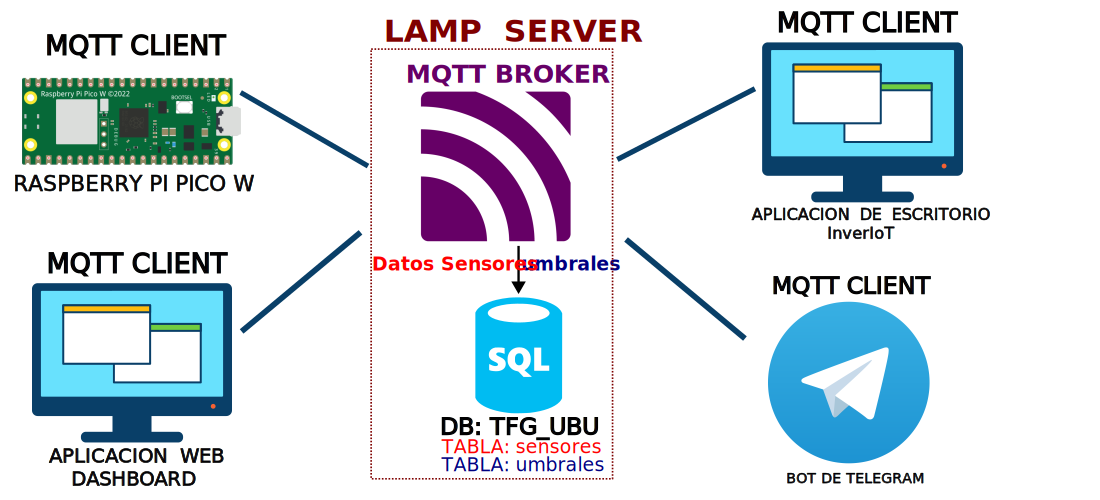
\includegraphics[width=1\textwidth]{img/diagramas/diagrama_general.png}
	\caption{Interacción entre cada parte del proyecto.} \label{Img:diagrama_general}
\end{figure}

Definimos umbrales (valor mínimo/máximo) para monitorizar cuando es que los valores de los sensores no están dentro de límites aceptables. En caso de detectar un valor anómalo fuera de estos umbrales, se genera una alerta.

\begin{table}[htbp]
\begin{center}
	\caption{Umbrales ideales para un invernadero de cannabis medicinal.}\label{tabla:umbrales}
\begin{tabular}{|l|l|l|l|}
\hline
\rowcolor[HTML]{C0C0C0} 
\textbf{Característica} & \textbf{Mínimo} & \textbf{Máximo} & \textbf{Unidades}\\ \hline
TEMPERATURA & 30 & 35 & \textcelsius\\ \hline
HUMEDAD & 30 & 70 & \% \\ \hline
LUMINOSIDAD & 30 & 150 & lux\\ \hline
HUMEDAD DEL SUELO & 20 & 80 & \% \\ \hline
\end{tabular}
\end{center}
\end{table}

%\begin{table}[htbp]
%\begin{center}
%\caption{Topics de MQTT usados.}
%\begin{tabular}{|l|l|} %|c|c|
%\hline
%\rowcolor[HTML]{C0C0C0} 
%\textbf{Nombre del topic} & \textbf{Descripción}\\ \hline
%invernadero/sensores & fecha, hora y valores de sensores \\ \hline
%invernadero/umbrales & valores límite \\ \hline
%invernadero/ordenes & Permite activar un mecanismo \\ \hline
%\end{tabular}
%\end{center}
%\end{table}

%A continuación veremos cada parte del proyecto para su mejor comprensión.

\subsection{Servidor LAMP}\label{proyecto:LAMP}

Opté por establecer un servidor LAMP para facilitar el envío y manejo de datos. La implementación de este servidor se llevó a cabo en el sistema operativo Ubuntu~\cite{misc:Ubuntu}, el cual fue virtualizado utilizando Hyper-V~\cite{manual:Hyper_V}.
En esta instancia, se emplea un servidor físico HP ProLiant~\cite{misc:HP_ProLiant} para la virtualización de los servicios Apache~\cite{misc:Apache}, MySQL~\cite{misc:Mysql}, PHP~\cite{misc:PHP} y SSH~\cite{misc:SSH}.

\begin{table}[htbp]
\begin{center}
\caption{Características del servidor HP ProLiant.}
\begin{tabular}{|l|l|}
\hline
\rowcolor[HTML]{C0C0C0} 
\textbf{Característica} & \textbf{Descripción}\\ \hline
Sistema operativo & Windows Server 2019 Standard\\ \hline
Fabricante & Hewlett Packard Enterprise \\ \hline
Modelo & Hewlett Packard Enterprise x64 Class PC\\ \hline
Procesador & Intel(R) Xeon(R) Silver 4210R CPU @ 2.4GHz 2.39GHz\\ \hline
Memoria instalada (RAM) & 128 GB (128 GB utilizable) \\ \hline
Tipo de sistema & Sistema operativo de 64 bits, procesador x64 \\ \hline
\end{tabular}
\end{center}
\end{table}

\begin{figure}[h]
	\centering
	\includegraphics[width=0.9\textwidth]{img/desarrollo/LAMP_servicios.png}
	\caption{Servicios instalados y operativos en el servidor LAMP.} \label{Img:LAMP_servicios}
\end{figure}

\subsection{NodeMqtt}\label{proyecto:NodeMqtt}

\textbf{NodeMqtt} es un servicio en Node.js~\cite{misc:Nodejs} que se ejecuta dentro del servidor LAMP, escucha los topics \textbf{invernadero/sensores} e \textbf{invernadero/umbrales}. Utiliza la librería MQTT.js~\cite{misc:MQTTjs}.

Está conformado por los siguientes archivos: index.js y package.json.

%\begin{itemize}
	%\item \textbf{index.js:}
		%Es el punto de entrada del código de la aplicación.
	%\item \textbf{package.json:}
		%Es un archivo de configuración que describe la aplicación y sus dependencias.
%\end{itemize}

Los datos son enviados por la placa Raspberry Pi Pico W RP2040~\cite{misc:RPiPicoW} usando MQTT, que recopila valores de sensores, y el servicio \textbf{nodeMqtt} captura los datos de los topics MQTT llamados \textbf{invernadero/sensores} e \textbf{invernadero/umbrales}, formatea y luego inserta estos datos en la base de datos MySQL~\cite{misc:Mysql} llamada \textbf{TFG\_UBU}.

La base de datos contiene dos tablas llamadas \textbf{sensores} y \textbf{umbrales}.

\begin{table}[htbp]
\begin{center}
	\caption{Columnas de las tablas contenidas en TFG\_UBU.}
\begin{tabular}{|l|l|}
\hline
\rowcolor[HTML]{C0C0C0} 
\textbf{sensores} & \textbf{umbrales}\\ \hline
fecha & temperatura\_minima \\ \hline
hora & temperatura\_maxima \\ \hline
temperatura & humedad\_ambiente\_minima \\ \hline
humedad & humedad\_ambiente\_maxima \\ \hline
intensidad\_luz & luminosidad\_minima \\ \hline
humedad\_suelo & luminosidad\_maxima \\ \hline
			   & humedad\_suelo\_minima \\ \hline
			   & humedad\_suelo\_maxima \\ \hline
			   & fecha\_actualización \\ \hline
\end{tabular}
\end{center}
\end{table}

\begin{figure}[h]
	\centering
	\includegraphics[width=1\textwidth]{img/diagramas/mqtt_nodeMqtt.png}
	\caption{MQTT con Node.js para almacenar datos de los sensores.}
\end{figure}

%\begin{figure}[h]
	%\centering
	%\includegraphics[width=0.1\textwidth]{img/desarrollo/mysql_tabla_sensores.png}
	%\caption{Data almacenada en la tabla \textbf{sensores}.}
%\end{figure}

\subsection{Hardware}\label{proyecto:Hardware}

Se optó por la Raspberry Pi Pico W debido a su eficiencia energética y coste accesible. Se conectaron al sistema un sensor de humedad y temperatura DHT22~\cite{manual:DHT22}, un sensor de intensidad de luz BH1750~\cite{manual:BH1750}, y un sensor de humedad de suelo~\cite{wiki:SensorHumedadSuelo}. Además, se incorporaron LEDs RGB~\cite{manual:LedRGB} para señalizar alertas.

\begin{figure}[h]
    \centering
    \includegraphics[width=1\textwidth]{img/diagramas/conexiones.png}
    \caption{Conexiones.} \label{Img:conexionesHardware}
\end{figure}

\begin{itemize}
	\item La Raspberry Pi Pico W estará situada en el invernadero para la recopilación de datos.
	\item Los LEDs RGB, instalados en la oficina del cliente, indicarán visualmente si los valores superan los umbrales establecidos.
	\item La pantalla OLED estará colocada en la puerta del invernadero para mostrar los valores actualizados.
\end{itemize}

Los datos se muestran en una pantalla OLED~\cite{manual:Oled} en tiempo real.

La Raspberry Pi Pico W establece conexión con el servidor LAMP a través de MQTT, facilitando la transmisión de los datos de los valores medidos por los sensores, el envío de umbrales predefinidos y la recepción de órdenes para ejecutar acciones específicas.

%\begin{figure}[h]
	%\centering
	%\includegraphics[width=0.5\textwidth]{img/fotos/conexiones_real.png}
	%\caption{Raspberry Pi Pico W y sensores conectados.} \label{Img:conexion_simple}
%\end{figure}

\begin{figure}[h]
	\centering
	\includegraphics[width=1\textwidth]{img/diagramas/mqtt_hardware.png}
	\caption{Conexión de la Raspberry Pi Pico W con el servidor LAMP.} \label{Img:mqtt_hardware}
\end{figure}

\begin{figure}[h]
	\centering
	\includegraphics[width=0.7\textwidth]{img/fotos/oled1.png}
	\caption{Pantalla oled conectada a la Raspberry Pi Pico W.} \label{Img:oled_conexion}
\end{figure}

%\begin{figure}[h]
	%\centering
	%\includegraphics[width=0.7\textwidth]{img/herramientas/rpipicow_umqtt.png}
	%\caption{Librería umqtt para conexión mediante MQTT.} \label{Img:rpipicow_umqtt}
%\end{figure}

\subsection{InverIoT}\label{proyecto:InverIoT}
Usando el lenguaje de programación C\#~\cite{manual:CSharp} y utilizando Windows Forms, se desarrolla una aplicación de escritorio para Windows al que se ha llamado InverIoT, que permite al usuario monitorizar el histórico de datos, y también visualizar los datos en tiempo real.

\begin{figure}[h]
    \centering
    \includegraphics[width=0.95\textwidth]{img/desarrollo/InverIoT_Desktop.png}
	\caption{Aplicación de escritorio \textbf{InverIoT}.}
\end{figure}

\begin{figure}[h]
    \centering
    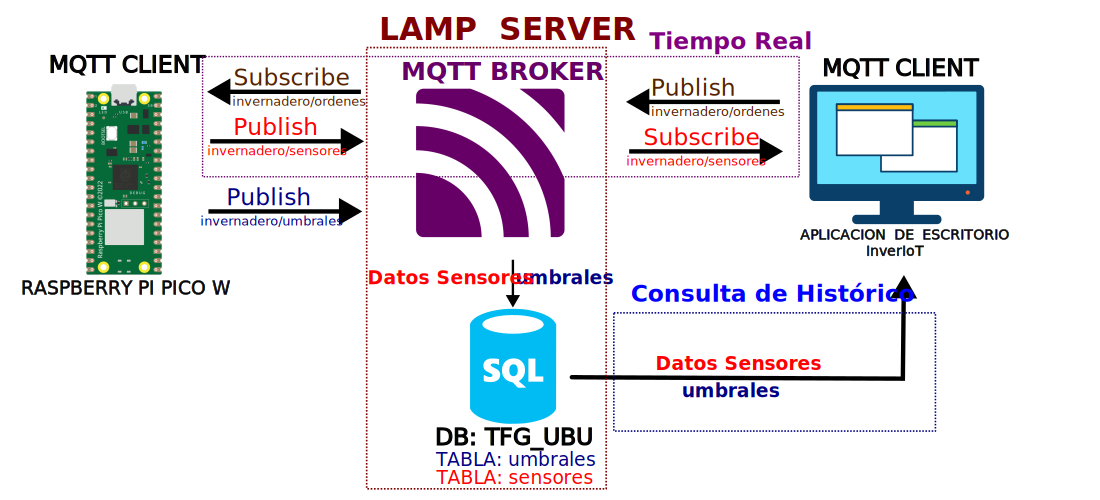
\includegraphics[width=1\textwidth]{img/diagramas/mqtt_InverIoT.png}
    \caption{Interacción entre la aplicación y el servidor LAMP.}
\end{figure}

Utilizando el protocolo MQTT~\cite{manual:MQTT}, la aplicación suscribe y recibe los datos publicados en el mismo tema. 

Para el histórico de datos no utiliza MQTT, se conecta al servidor LAMP mediante Mysql Protocol y extrae la data de la base de datos llamada \textbf{TFG\_UBU}.

\begin{figure}[h]
    \centering
    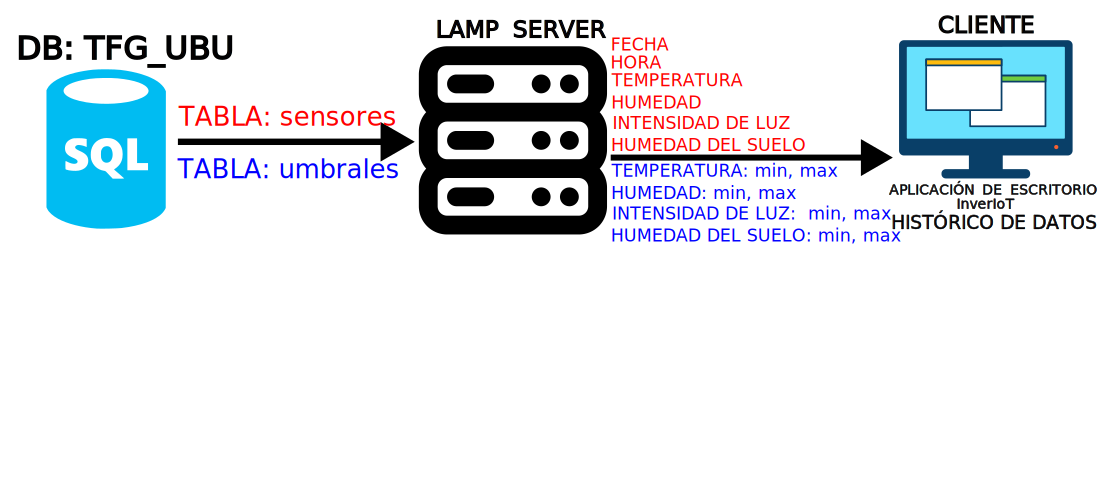
\includegraphics[width=1\textwidth]{img/diagramas/mqtt_InverIoT_Historico.png}
    \caption{Datos usados para mostrar el histórico de datos.}
\end{figure}


Estos datos son formateados y presentados en textboxes correspondientes, con unidades de medida agregadas.

Se incorporan botones para activar o desactivar mecanismos, esto es representado prendiendo o apagando un LED verde, recordar que hay un led RGB por cada variable medida.


\begin{figure}[h]
    \centering
    \includegraphics[width=1\textwidth]{img/desarrollo/InverIoT_Desktop_botones_control.png}
	\caption{Botones para activar o desactivar mecanismos.}
\end{figure}

\begin{figure}[h]
	\centering
	\includegraphics[width=0.85\textwidth]{img/desarrollo/InverIoT_verde_clickMecanismo.png}
	\caption{Activación de un mecanismo mediante un clic.}\label{img:InverIoTBotones}
\end{figure}

\begin{figure}[h]
	\centering
	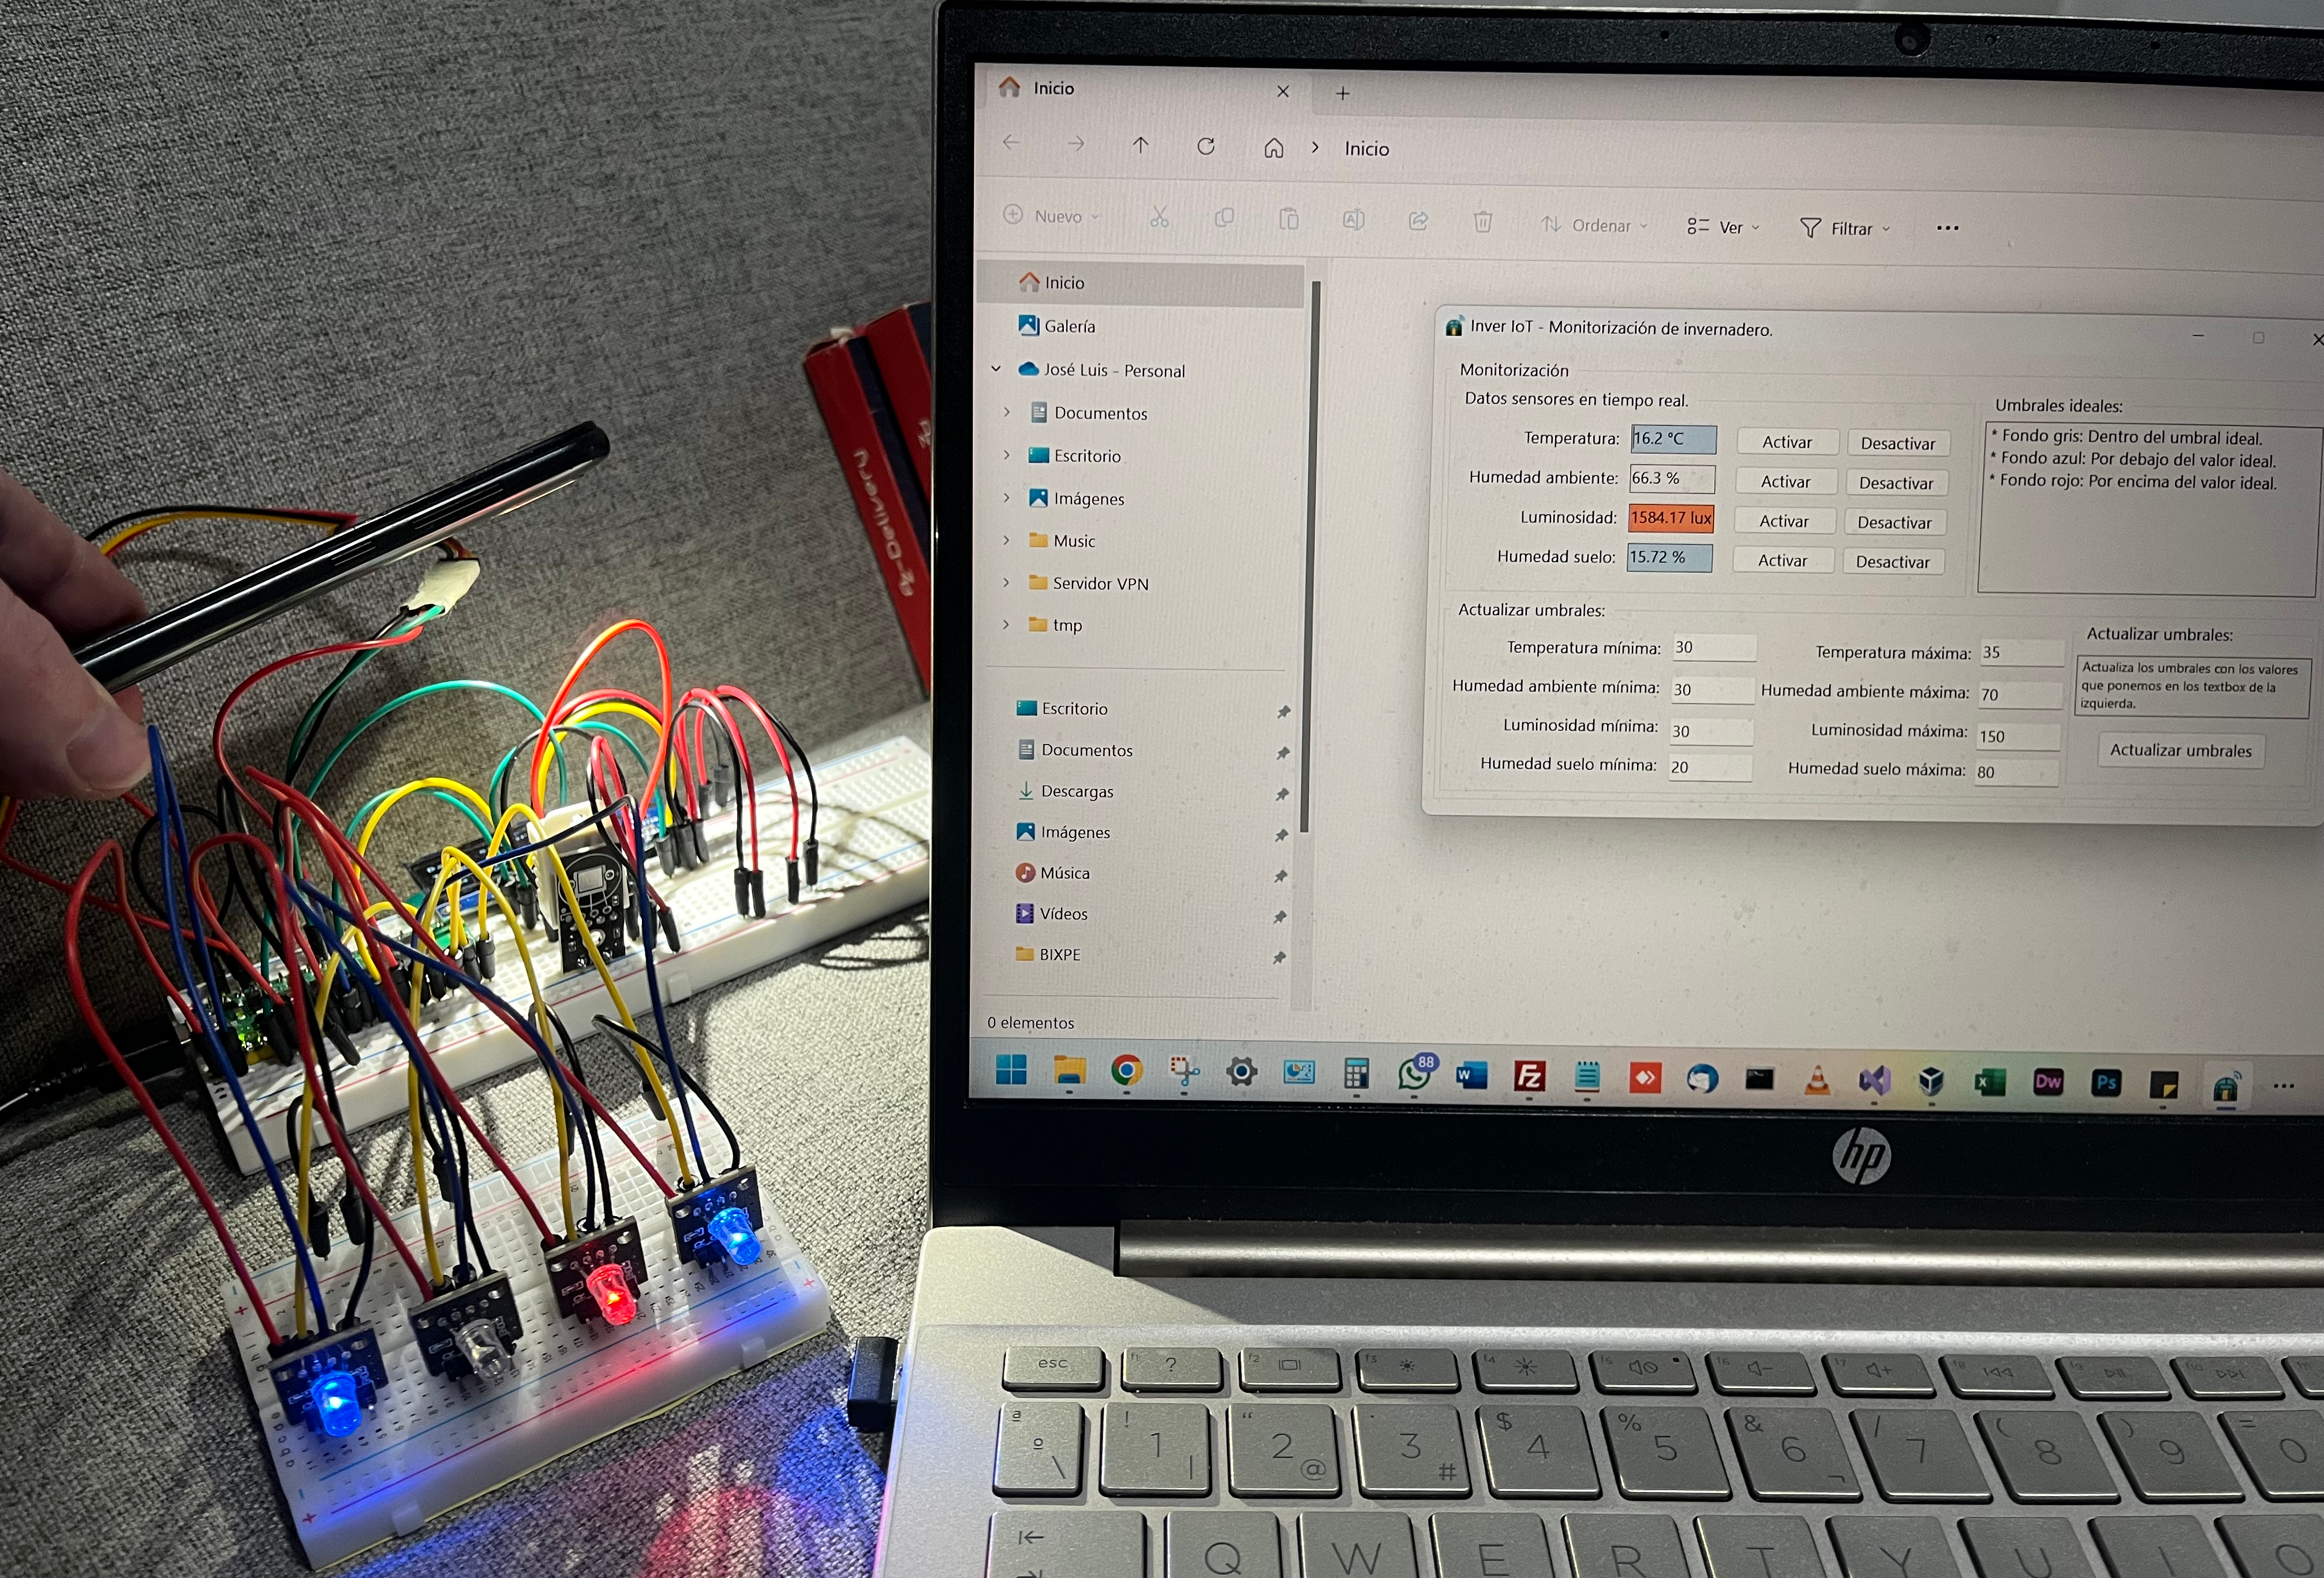
\includegraphics[width=0.85\textwidth]{img/fotos/InverIoT_PasandoUmbralLuz.png}
	\caption{Aplicación indicando que se ha sobrepasado el umbral de luz.}\label{img:InverIoTPasandoUmbralLuz}
\end{figure}

En la imagen \ref{img:InverIoTBotones} se puede observar 8 textboxes en la parte inferior para ajustar manualmente los valores mínimos y máximos de cada parámetro. Inicialmente estos valores fueron extraídos de la base de datos en el servidor LAMP.

En la imagen \ref{img:InverIoTPasandoUmbralLuz} se está sometiendo al sensor de intensidad de luz a sobrepasar el umbral establecido, el led rojo indica eso. Si un valor está por debajo del umbral, se indicará mediante el led de color azul. Se puede observar tal acontecimiento de colores en el hardware y en la aplicación de escritorio.

\begin{figure}[h]
    \centering
    \includegraphics[width=0.95\textwidth]{img/desarrollo/InverIoT_Histórico.png}
    \caption{Historial de los datos mostrada en la aplicación.}
\end{figure}


\begin{figure}[h]
    \centering
    \includegraphics[width=0.95\textwidth]{img/desarrollo/InverIoT_Gráficas.png}
    \caption{Gráfica mostrando los datos en un intervalo de fechas.}
\end{figure}




\pagebreak

\subsection{Dashboard}\label{proyecto:Dashboard}
Se ha creado un dashboard web con Node.js que habilita al usuario para visualizar en tiempo real los datos capturados por los sensores y acceder a un historial con filtro de fecha. La interfaz presenta similitudes con la aplicación de escritorio para mantener una experiencia coherente.

Los valores que exceden los umbrales establecidos se destacan mediante cambios de color.

\begin{figure}[h]
    \centering
    \includegraphics[width=0.95\textwidth]{img/desarrollo/Dashboard1.png}
    \caption{Intensidad de luz superando los umbrales.} \label{Img:Dashboard1}
\end{figure}

La plataforma incluye una gráfica en tiempo real y la capacidad de acceder a un historial con filtro de fecha.

\begin{figure}[h]
    \centering
    \includegraphics[width=0.95\textwidth]{img/diagramas/mqtt_dashboard.png}
    \caption{Dashboard web interactuando con el servidor LAMP.} \label{Img:mqtt_dashboard}
\end{figure}

La imagen \ref{Img:mqtt_dashboard} ilustra de manera significativa el uso de MQTT para la obtención de datos en tiempo real. Cabe destacar que, además, se utiliza el protocolo MySQL para extraer información de la base de datos alojada en el servidor LAMP, permitiendo así mostrar el histórico de datos

\begin{figure}[h]
    \centering
    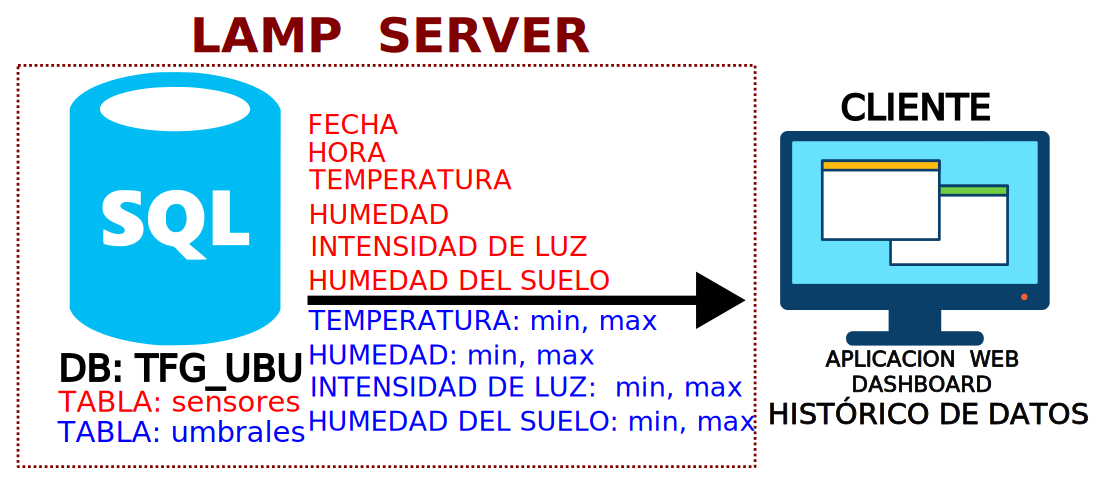
\includegraphics[width=1\textwidth]{img/diagramas/mqtt_dashboard_Historico.png}
    \caption{Valores específicos extraídos de la base de datos.} \label{Img:Dashboard_diagrama_Historico}
\end{figure}

\begin{figure}[h]
    \centering
    \includegraphics[width=0.95\textwidth]{img/desarrollo/Dashboard_Historico.png}
    \caption{Vista del historial, al cargar, muestra los datos del día actual.} \label{Img:Dashboard_Historico}
\end{figure}

%\begin{figure}[h]
    %\centering
    %\includegraphics[width=1\textwidth]{img/diagramas/mqtt_dashboard_TiempoReal.png}
    %\caption{Mediante MQTT extrae los datos para mostrarlos en tiempo real.} \label{Img:Dashboard_diagrama_TiempoReal}
%\end{figure}

El panel de control está disponible para su acceso a través del siguiente enlace: \href{http://www.inveriot.com}{InverIoT Dashboard}


%\begin{figure}[h]
	%\centering
	%\includegraphics[width=1\textwidth]{img/desarrollo/Dashboard2.png}
	%\caption{Página Web \href{http://www.inveriot.com}{InverIoT} desarrollada con Node.js.}
%\end{figure}

%\begin{figure}[h]
	%\centering
	%\includegraphics[width=1\textwidth]{img/desarrollo/Dashboard3.png}
	%\caption{Página Web \href{http://www.inveriot.com}{InverIoT} desarrollada con Node.js.}
%\end{figure}
%En este contexto, detallaré la configuración del servidor y la implementación de Node.js en la página web.

\subsection{Bot de Telegram}\label{proyecto:BotTelegram}

Se implementó la funcionalidad de enviar alertas a través de Telegram en caso de que los valores recopilados excedieran los umbrales ideales~\ref{tabla:umbrales}.

Para esta función, empleamos un bot de Telegram~\cite{misc:Telegram_bots} que envía mensajes de alerta si alguno de los valores está fuera del umbral establecido. 

La creación del bot se hace utilizando BotFather\cite{misc:BotFather} que es un bot especial en la plataforma de mensajería Telegram~\cite{misc:Telegram} que permite a los usuarios crear y gestionar sus propios bots. Al interactuar con BotFather, los usuarios pueden definir el nombre, la descripción, la imagen y otras configuraciones de su bot. Además, BotFather proporciona un token único para cada bot creado, el cual se utiliza para autenticar las solicitudes y permitir la interacción entre el bot y la plataforma de Telegram.

Para este proyecto el nombre del bot creado es \textbf{InverIoTBot}.

\begin{figure}[h]
	\centering
	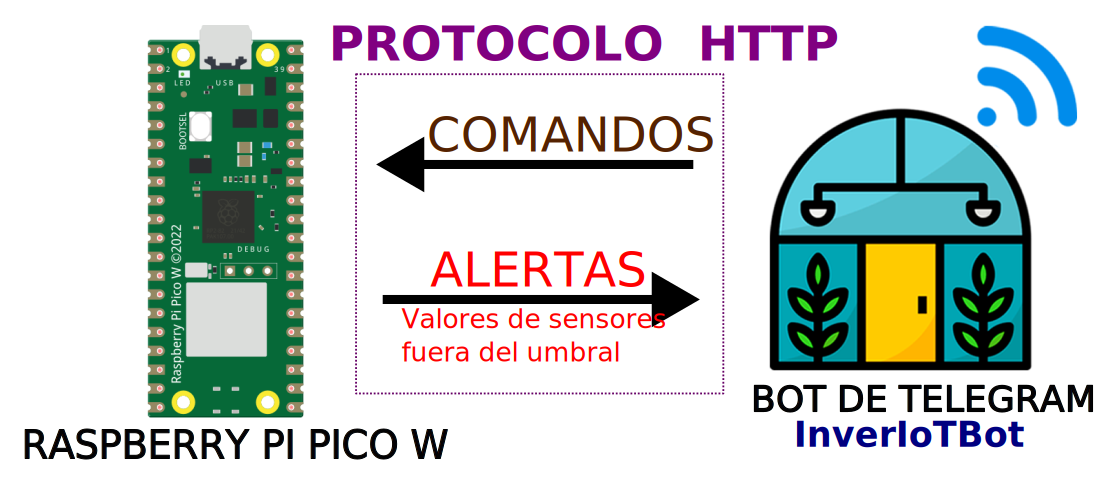
\includegraphics[width=1\textwidth]{img/diagramas/telegramBot.png}
	\caption{La interacción es mediante protocolo HTTP.} \label{Img:telegramBot}
\end{figure}

El bot también brinda la posibilidad de enviar comandos para acciones específicas, como obtener el valor de un sensor o activar un mecanismo vinculado a un sensor en particular.

Tener presente que la activación de un mecanismo se representa encendiendo un LED de color verde, y cada sensor está asociado a un LED RGB específico.
 
\begin{table}[htbp]
\begin{center}
\caption{Comandos del bot para la consulta de los datos.}
\begin{tabular}{|l|l|} %|c|c|
\hline
\rowcolor[HTML]{C0C0C0} 
\textbf{Comando} & \textbf{Valor que retorna}\\ \hline
/temp & Temperatura del ambiente\\ \hline
/huma& Humedad del ambiente \\ \hline
/lum & Luminosidad\\ \hline
/hums & Humedad del suelo\\ \hline
/todos & Todos los valores de los sensores\\ \hline
\end{tabular}
\end{center}
\end{table}


\begin{table}[htbp]
\begin{center}
\caption{Comandos del bot para activar un mecanismo.}
\begin{tabular}{|l|l|} %|c|c|
\hline
\rowcolor[HTML]{C0C0C0} 
\textbf{Comando} & \textbf{Acción específica}\\ \hline
/t\_ON & Mecanismo de temperatura prendido\\ \hline
/t\_OFF & Mecanismo de temperatura apagado\\ \hline
/ha\_ON & Mecanismo de humedad del ambiente prendido\\ \hline
/ha\_OFF & Mecanismo de humedad del ambiente apagado\\ \hline
/l\_ON & Mecanismo de luminosidad prendido\\ \hline
/l\_OFF & Mecanismo de luminosidad apagado\\ \hline
/hs\_ON & Mecanismo de humedad del suelo prendido\\ \hline
/hs\_OFF & Mecanismo de humedad del suelo apagado\\ \hline
\end{tabular}
\end{center}
\end{table}

\begin{figure}[h]
	\centering
	\includegraphics[width=0.7\textwidth]{img/desarrollo/BotTelegram_alertas.png}
	\caption{Alertas del bot de Telegram.} \label{Img:BotTelegram_alertas}
\end{figure}

\begin{figure}[h]
	\centering
	\includegraphics[width=0.7\textwidth]{img/desarrollo/BotTelegram_comandos.png}
	\caption{Consulta a la base de datos mediante comandos usando Telegram.}
\end{figure}
